\section{Design Space Exploration}

After we fixed the basic architectures of the design. We can try different HLS
knobs to optimize our accelerator from area and latency directions. \\

\subsection{Low Area Optimization}

\subsubsection{Customize PLM}

We want to customize PLM size for two different input variables. k-space
variables have the same size while sampling-space variables have the same size
but different from the k-space variables. So we set different PLMs for these two
groups. \\ \\ Since we can customize number of ports for each PLM, we shouldn't
waste any ports in order to save area. For PLMs storing input data, we set the
number of writing ports accordingly to be consistent with DMA width. For
example, if DMA width is 64, while data width is 32, then there are two writing
ports. If DMA width and data width are both 32, then we only need one writing
ports. The number of reading ports of different PLMs depends on the parallelism
level. If parallelism level is 4, we need to read 4 k-variables in parallel in
the compute\_kernel process. So 4 reading ports are needed.\\

\subsubsection{Fixed-Point Datatype Optimization}

The MRI-Q accelerator deals with fixed point datatype. We can reduce fixed point
precision to reduce both latency and area. When we have only one type of
fixed-point data representation and reduce the word length to 29, there are no
errors in output data and both area and latency reduced. Further reduction in
word length led to output errors. In order to further reduce the data width of
the fixed-point representation, I analyzed all the testing data provided by the
Parboil benchmark suite. Some data are bound to be very small value, for
example, the output of trigonometric functions is always less than 1, and some
are large values. The range of data are shown in Table.\ref{tab-8}. I set two
different fixed-point representations, shown in Table.\ref{tab-4}. We use
FPDATA\_S to represent kx, ky, kz, phiR, phiI, x, y, z, and phiMag, sinArg,
cosArg. And we use FPDATA\_L to represent the other variables. The result shows
that the error rate is 0.17\% when error threshold (percentage difference
between computed output and golden output), is set as 5\%. So the data width can
be as small as 24 compared to 32. \\

\begin{table}[h!]
    \centering
    \begin{tabular}{c|c|c|c}
    \hline
        & WL & IL & Fractional Bits \\
        \hline
   FPDATA\_S &  24  & 5  & 19 \\ 
FPDATA\_L &  24 & 11   & 13\\
    \hline
    \end{tabular}
    \caption{Fixed-point data representation}
    \label{tab-4}
\end{table}

\begin{table}[ht!]
    \centering
    \begin{tabular}{c|c|c|c}
    \hline \hline
   Variables &       Max&    Min& Integer bits\\
   \hline \hline
 x&     3.083235        &-0.500000& 3 \\
 y&     0.484375        &-0.500000& 1 \\
 z&     0.484375        &-0.500000& 1 \\
 kx&    10.889303       &-10.889303& 5 \\
 ky&    16.019472       &-16.019472& 5 \\
 kz&    0.585179        &-0.585179& 1\\
 phiI   &0.484375       &0.312500& 0 \\
 phiR   &0.484375       &0.406250& 0 \\
 phiMag &0.469238       &0.262695& 0 \\
 cosArg&        1.000000        &-1.000000& 2\\
 sinArg &1.000000       &-1.000000& 2 \\
 \hline
 expArg &226.168869     &-226.168869& 9 \\
 Qracc  &961.000000     &-472.693146& 11 \\
 Qiacc  &97.710320      &-97.710320& 8 \\
\hline \hline
    \end{tabular}
    \caption{Value range for all variables}
    \label{tab-8}
\end{table}

We experimented with small data set and we extracted area from the synthesized
RTL and extracted latency data from RTL simulation. This small dataset has numX
as 4 and numK as 16, and it is running with accelerator A0\_P4\_DMA64. The
extracted area and latency data are shown in Table.\ref{tab-3}. Area reduces by
31.5\%. Latency also reduces by 11.49\%. But when we simulate the bare-metal
application, it doesn't support data width as 24. So we set FPDATA\_S and
FPDATA\_L with the same specification (WL, IL) = (32, 12) in the other
evaluations.  \\

\begin{table}[h!]
    \centering
    \begin{tabular}{c|c|c|c}
    \hline
        & $WL=32$ & $WL=24$ &  Gain \\
        \hline
   area &  0.1185  & 0.0812   & -31.50\% \\ 
latency (ns) &  1740 &  1540  & -11.49\% \\
    \hline
    \end{tabular}
    \caption{Performance of FP precision reduction}
    \label{tab-3}
\end{table}

\subsection{Low Latency Optimization}

We have two directions to reduce latency. The first one is to accelerate the
loading and storing process. The second one is to accelerate the
computation. Since the data transportation between processor and the accelerator
is done in serial, we can increase the burst rate and DMA width. In our case,
burst rate is fixed and the DMA width is determined by the processor core we
have in our SoC. The Ariane core provides DMA width as 64-bit, while Leon3 core
has DMA width as 32-bit. In the computation phase, we can do loop unrolling and
loop pipeline to accelerate. Since we don't have the choice to work on
accelerating load and store process, we can only work on the
compute\_kernel. \\ \\
%
A0 architecture loads all the k-space data into PLM. It uses ping pong buffer to
load sampling space data. The RTL simulation waveform of A0\_P4\_DMA64 shows
that loading one batch of sampling space data takes 2 $\mu$s with batch\_size\_x
set as 128, and generating one pair of output data takes 7 $\mu$s . Thus
generating 128 pairs of output data takes 900 $\mu$s. So the compute\_kernel
process is dominating other processes, and the loading process of the sampling
space data is totally hidden by computation process. It also means that the
acceleration done on compute\_kernel will have the biggest impact on the final
latency. But A1 architecture behaves very differently. When we set
batch\_size\_k as 1024, loading five k-space variables takes 25 $\mu$s. If
num\_batch\_k was 10, then preparing all the input to generate one pair of
output takes $25\mu$s $* 10 = 250\mu$s, while the computation takes 7us to
finish. Loading process is dominating for A1 architecture and any optimization
to the compute\_kernel won't work. \\ \\
%
First, let's look at the Pareto curve of A0 architecture, which is shown in
Fig.\ref{fig-paral}. The area and latency data is extracted from RTL synthesis
results and RTL simulation results. The testing parameters are shown in Table
\ref{tab-test-param}. The number in P-<number> indicates the unroll-factor. We
can see that latency is decreasing when we increase the parallelism level. We
have tried unroll factor 4, 8, 16. In the compute\_kernel process, we have three
tasks which can be pipelined. The first one is to read data from PLMs to
registers. The second task is to do computation, and the third task is to store
the computed results. For our MRI-Q application, the third step is to accumulate
the intermediate results. Every task can be unrolled for unroll-factor number of
times. In order to support reading from the same PLM for unroll-factor number of
data into registers in parallel , the PLM in question should have unroll-factor
number of reading ports.

\begin{table}[h!]
     \centering
     \begin{tabular}{c|c|c}
        \hline
          Configurable variables& A0 & A1  \\
         \hline
         numX & 256 & 256 \\
         \hline
         batch\_size\_x & 128 & 128 \\
         \hline
         num\_batch\_x & 2 & 2 \\
          \hline
         numK & 3072 & 3072 \\  
         \hline
         batch\_size\_k & 3072 & 1024 \\
         \hline
         num\_batch\_x & 1 & 3 \\
         \hline
     \end{tabular}
     \caption{Testing Parameters of the Pareto curve}
     \label{tab-test-param}
 \end{table}

\begin{figure}[h!]
    \centering
    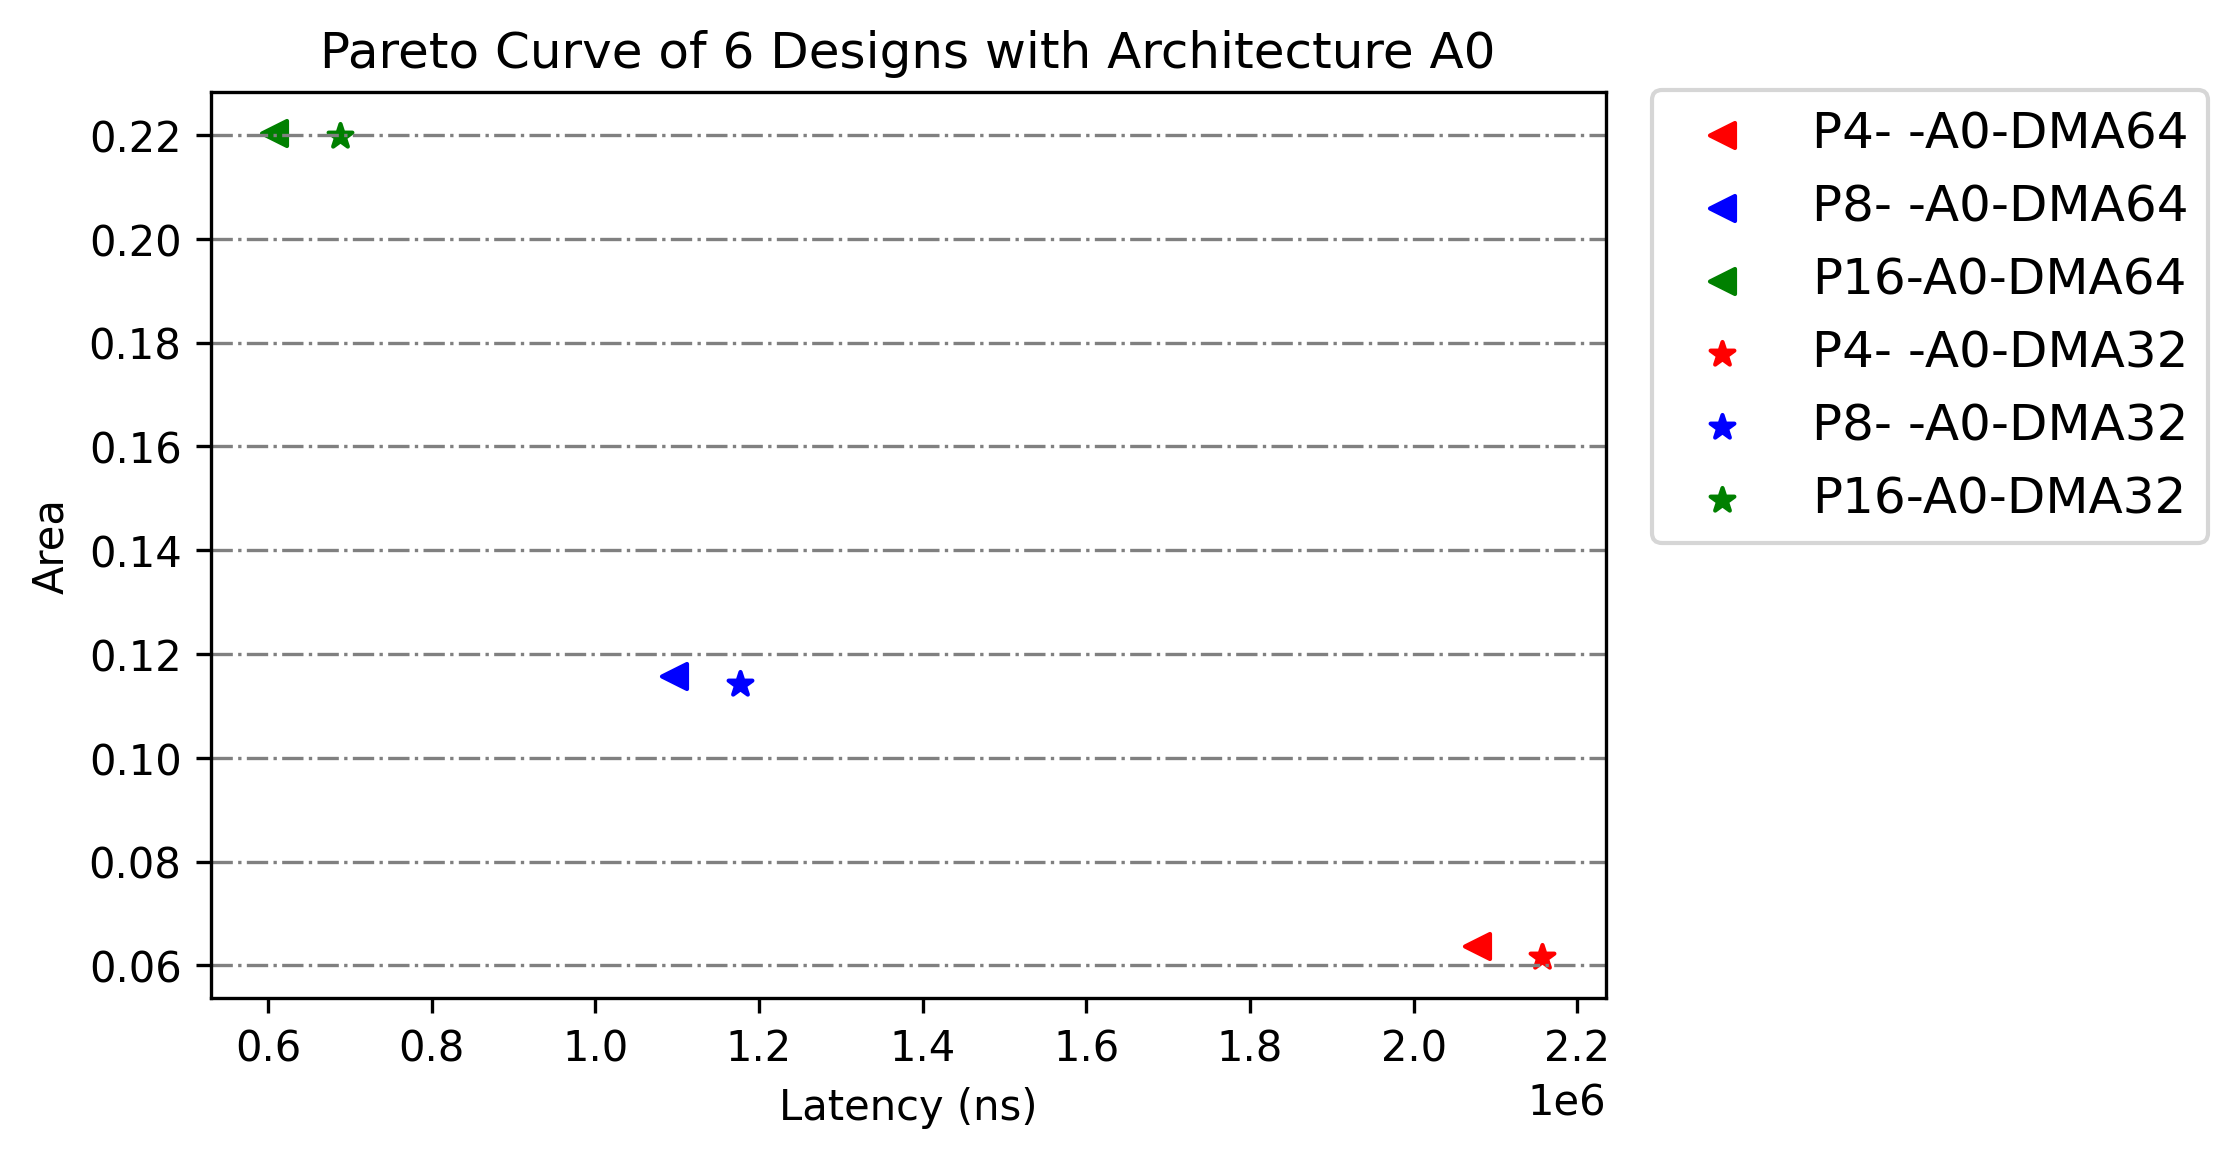
\includegraphics[width=\columnwidth]{figures/Pareto-curve-A0.png}
    \caption{Pareto curve of 6 designs of A0}
    \label{fig-paral}
\end{figure}

The latency optimization for A1 architecture should solely depend on the DMA
width as we have discussed above. The optimization done in compute\_kernel
shouldn't have any effect, shown in Fig.\ref{fig-a1-pareto}.\\

\begin{figure}[h!]
    \centering
    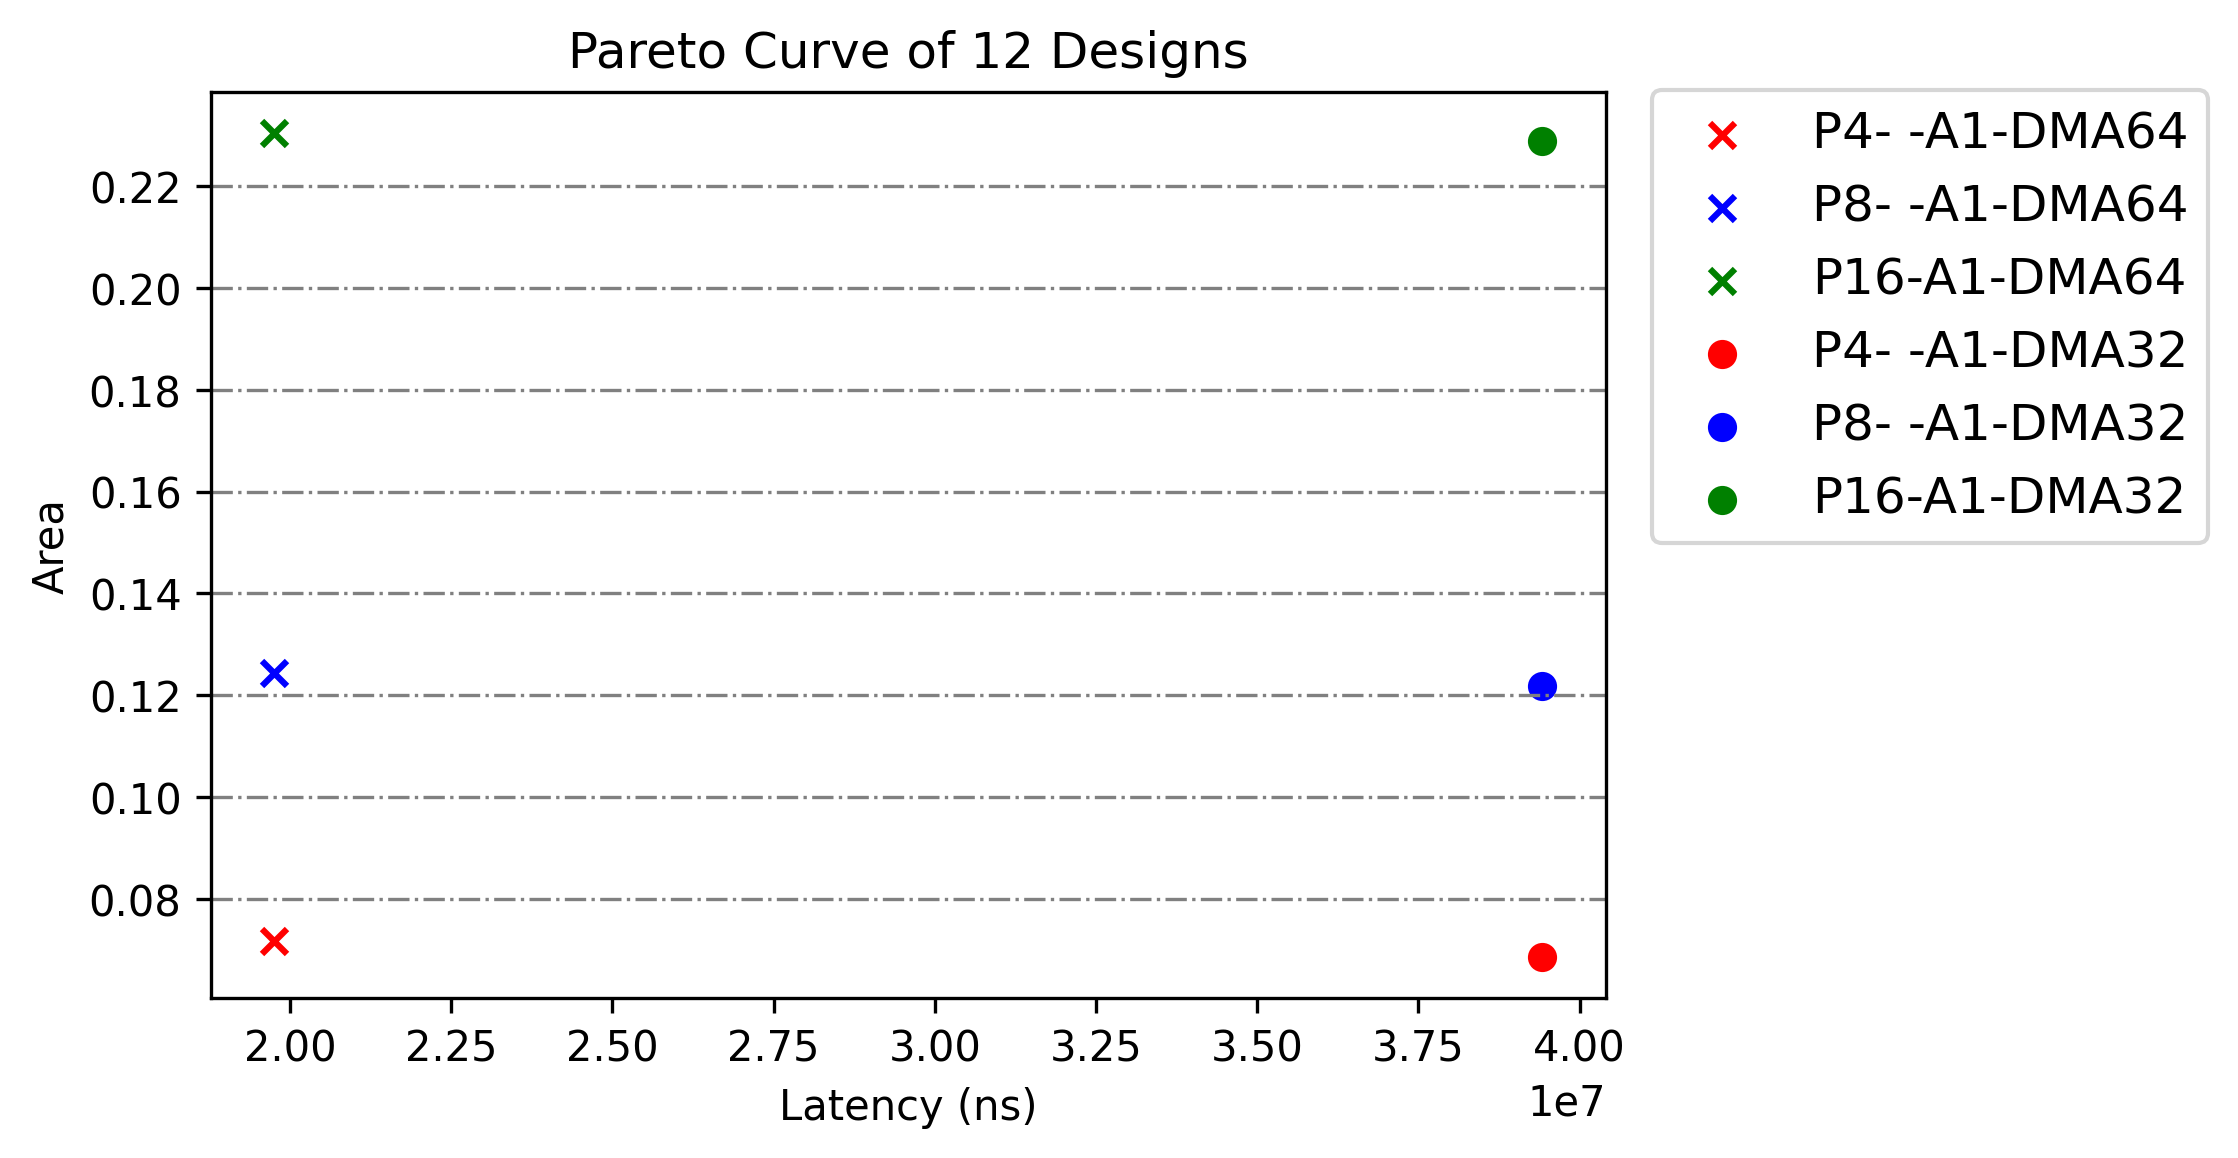
\includegraphics[width=\columnwidth]{figures/Pareto-curve-A1.png}
    \caption{Pareto curve of 6 designs of A1}
    \label{fig-a1-pareto}
\end{figure}



\subsection{Results of Testing on FPGA}

By invoking linux on FPGA, we collected both the software execution time running
on the Ariane core and the execution time running on the MRI-Q accelerator. For
A0 architecture, data is shown in Fig.\ref{fig-d32-64} for 32x32x32 (D32) and
64x64x64 (D64) dataset.  The right y-axis shows the speed-up of the two
testing. The speed up is greater than 5000 for both datasets when parallelism
level is 16. The testing result of D32 shows a slightly higher speed-up than D64
is because that numK of D32 is 1.5X of D64. Increasing parallelism in compute
can improve latency, same as the extracted data from the synthesized RTL.\\

\begin{figure}[h!]
    \centering
    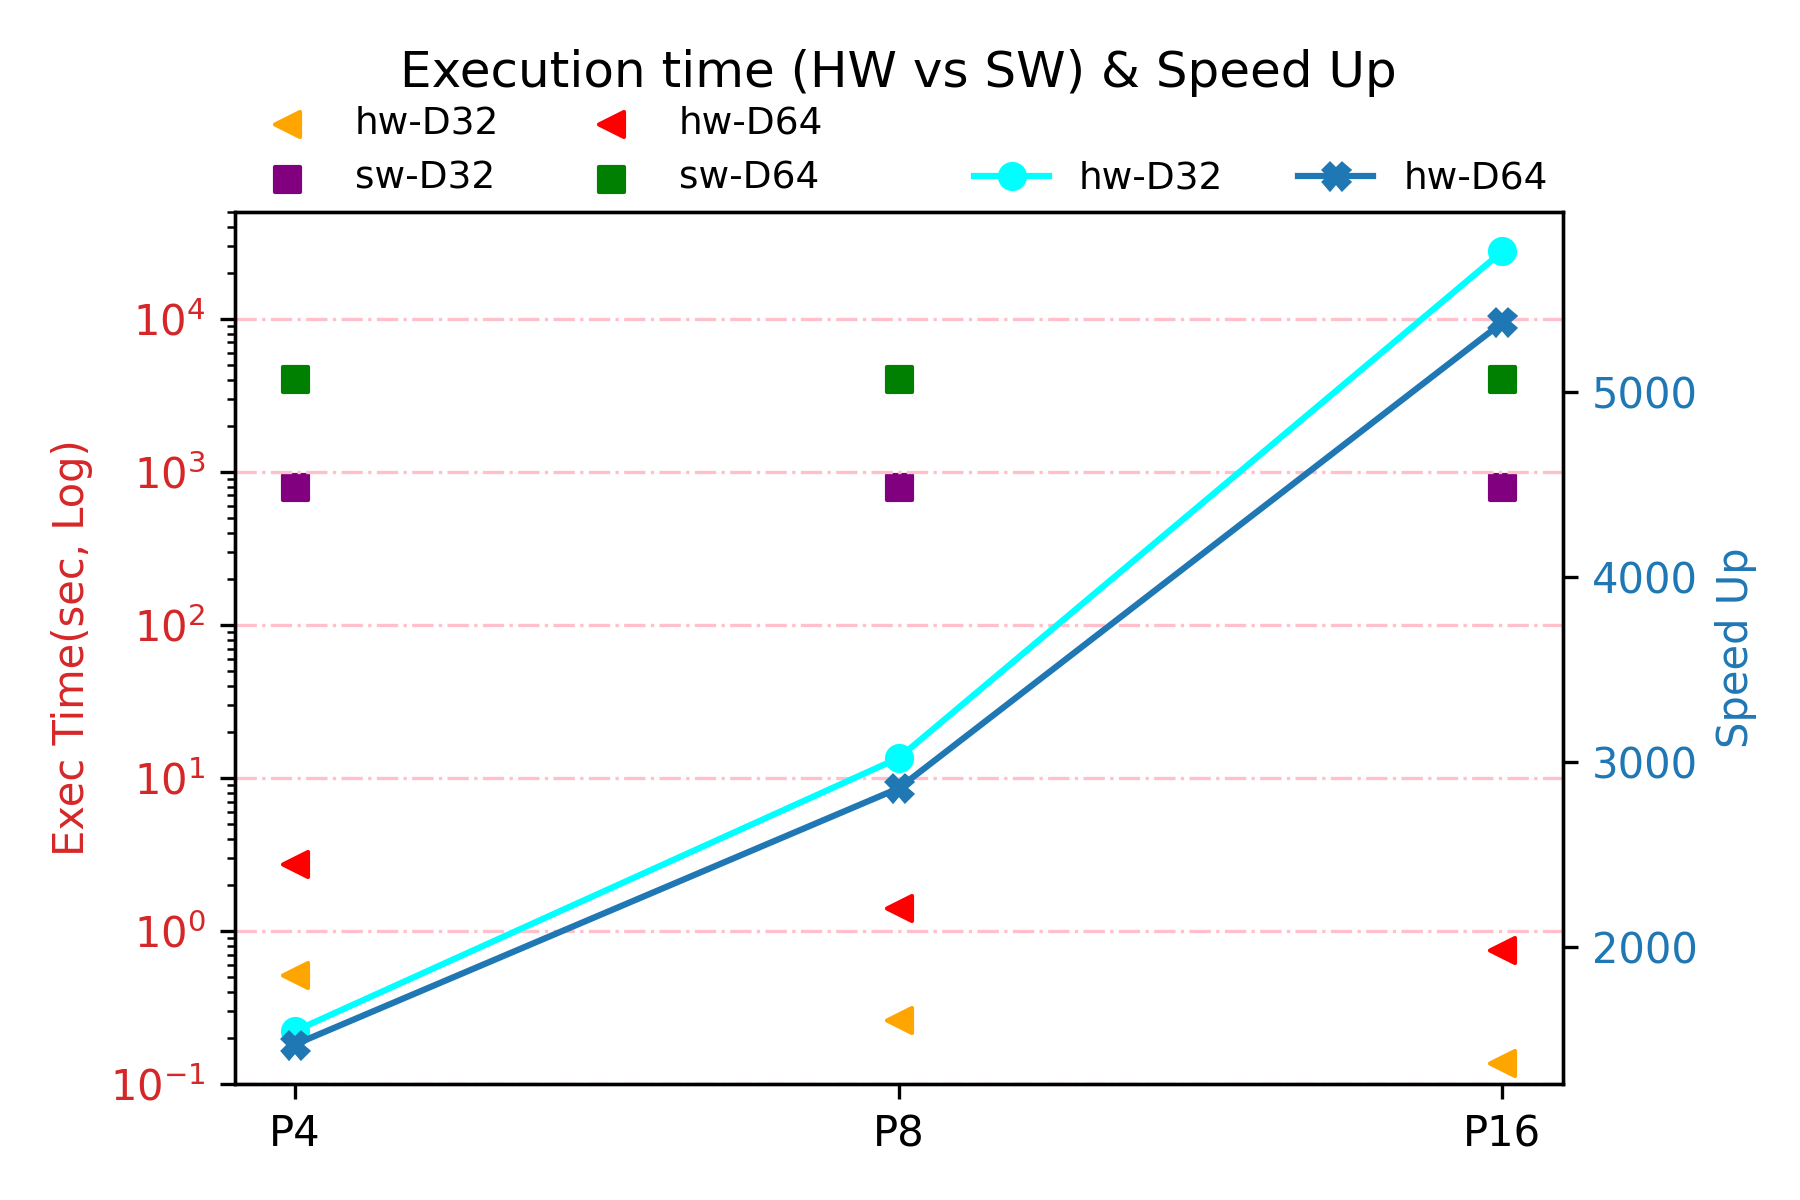
\includegraphics[width=\columnwidth]{figures/a0-both.png}
    \caption{Latency comparison of D32 and D64 Dataset}
    \label{fig-d32-64}
\end{figure}

For A1 architecture, latency results are shown in Fig.\ref{fig-a1-x} and
Fig.\ref{fig-a1-k}. For 128x128x128 dataset, numX = numK = 2048K. To evaluation
the speedup of accelerator with A1 architecture, I tested P4\_A1\_DMA64. As we
discussed in section 3.3, parallel level in compute process won't affect latency
performance, so we choose the P4 accelerator. (It is possible that there is a
parallelism level which is smaller than 4 and can also balance the loading and
computing processes to further reduce area while with the same latency
performance.).The speed-up value is increasing when increasing the data
size. Fig.\ref{fig-a1-x} shows the execution time comparison of software and
hardware and speedup when numK is fixed at 4K and numX is
increasing. Fig.\ref{fig-a1-k} shows how execution time and speedup change over
numK increasing from 4K to 256K while numX is fixed as 4.  At some point,
speedup saturates when numK and numX increases. For our A1 architecture, we get
at least 400 times acceleration compared with software execution for any
arbitrary input image size.\\

\begin{figure}[h!]
    \centering
    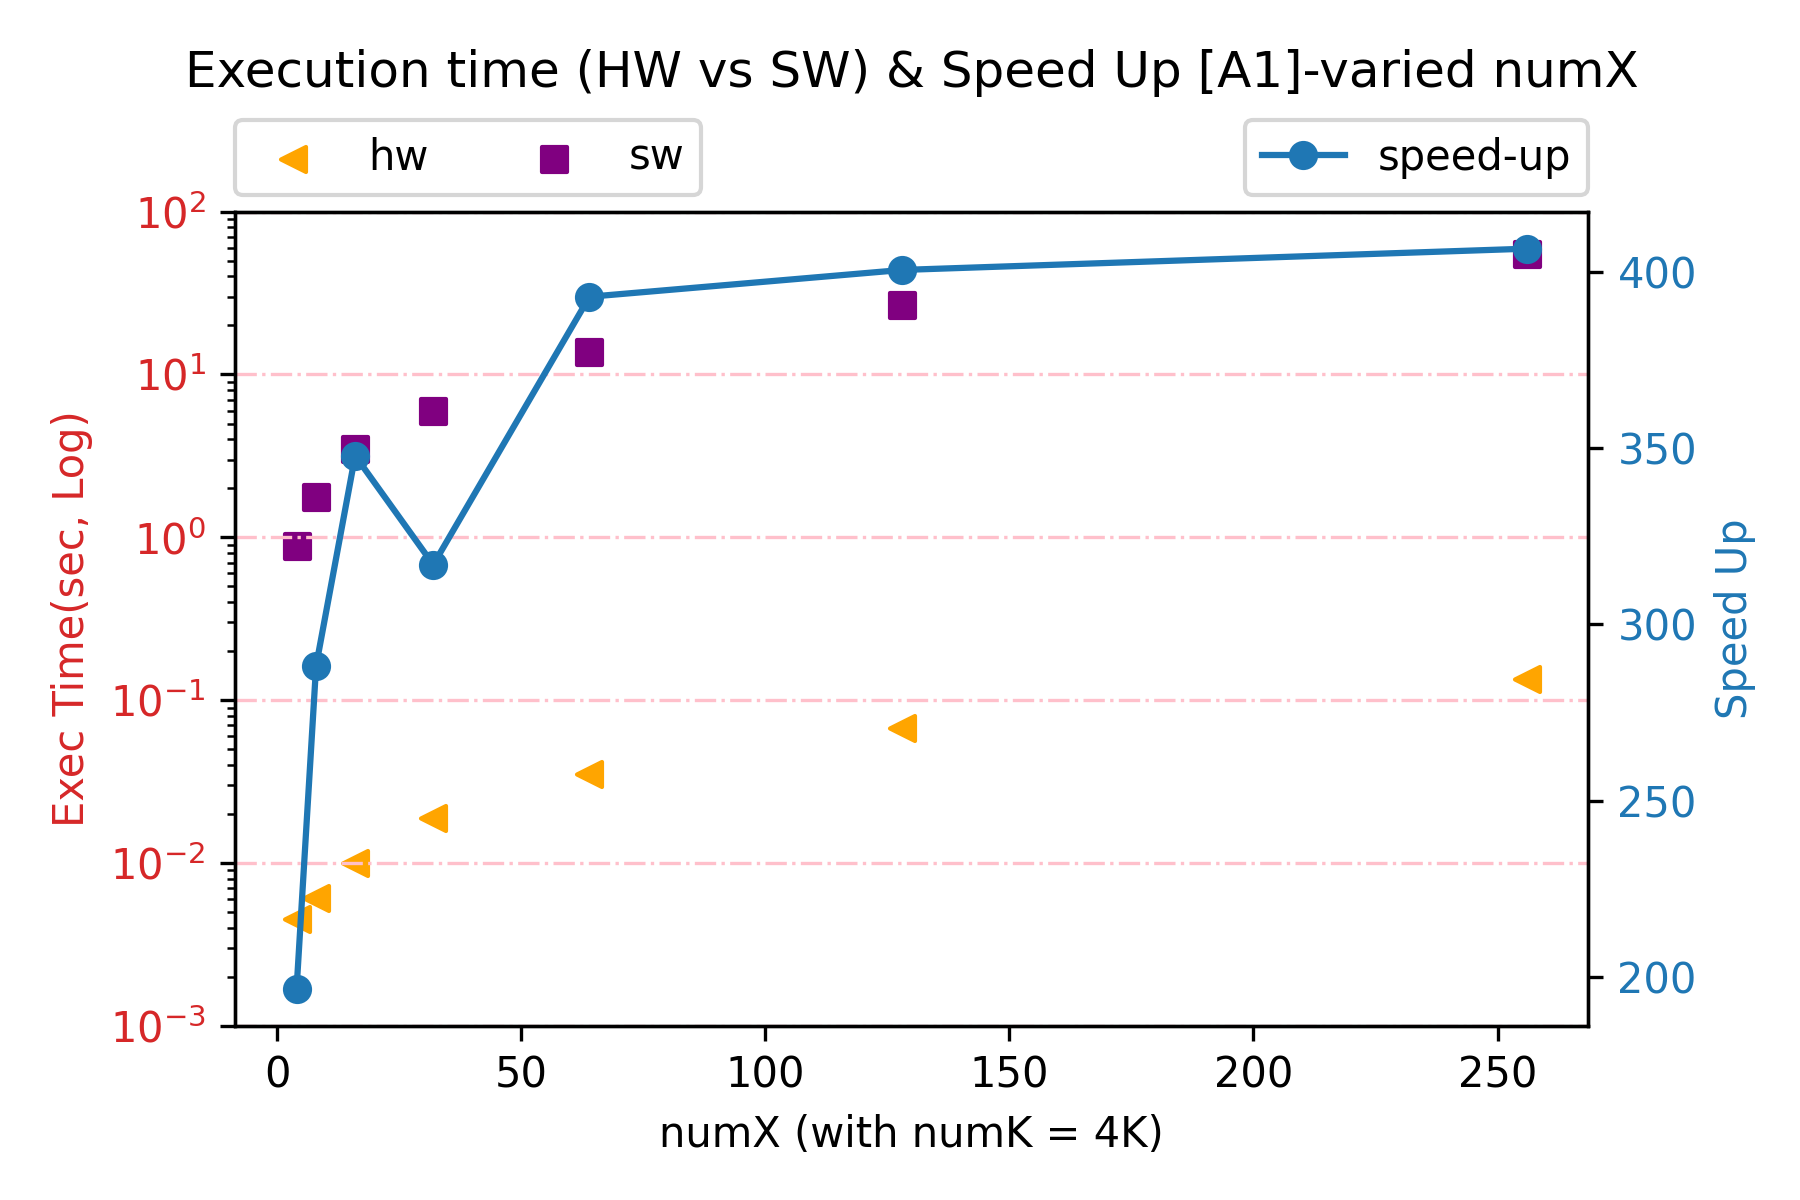
\includegraphics[width=\columnwidth]{figures/a1-vary-x.png}
    \caption{Latency with varying numX (numK=4K)}
    \label{fig-a1-x}
\end{figure}

\begin{figure}[h!]
    \centering
    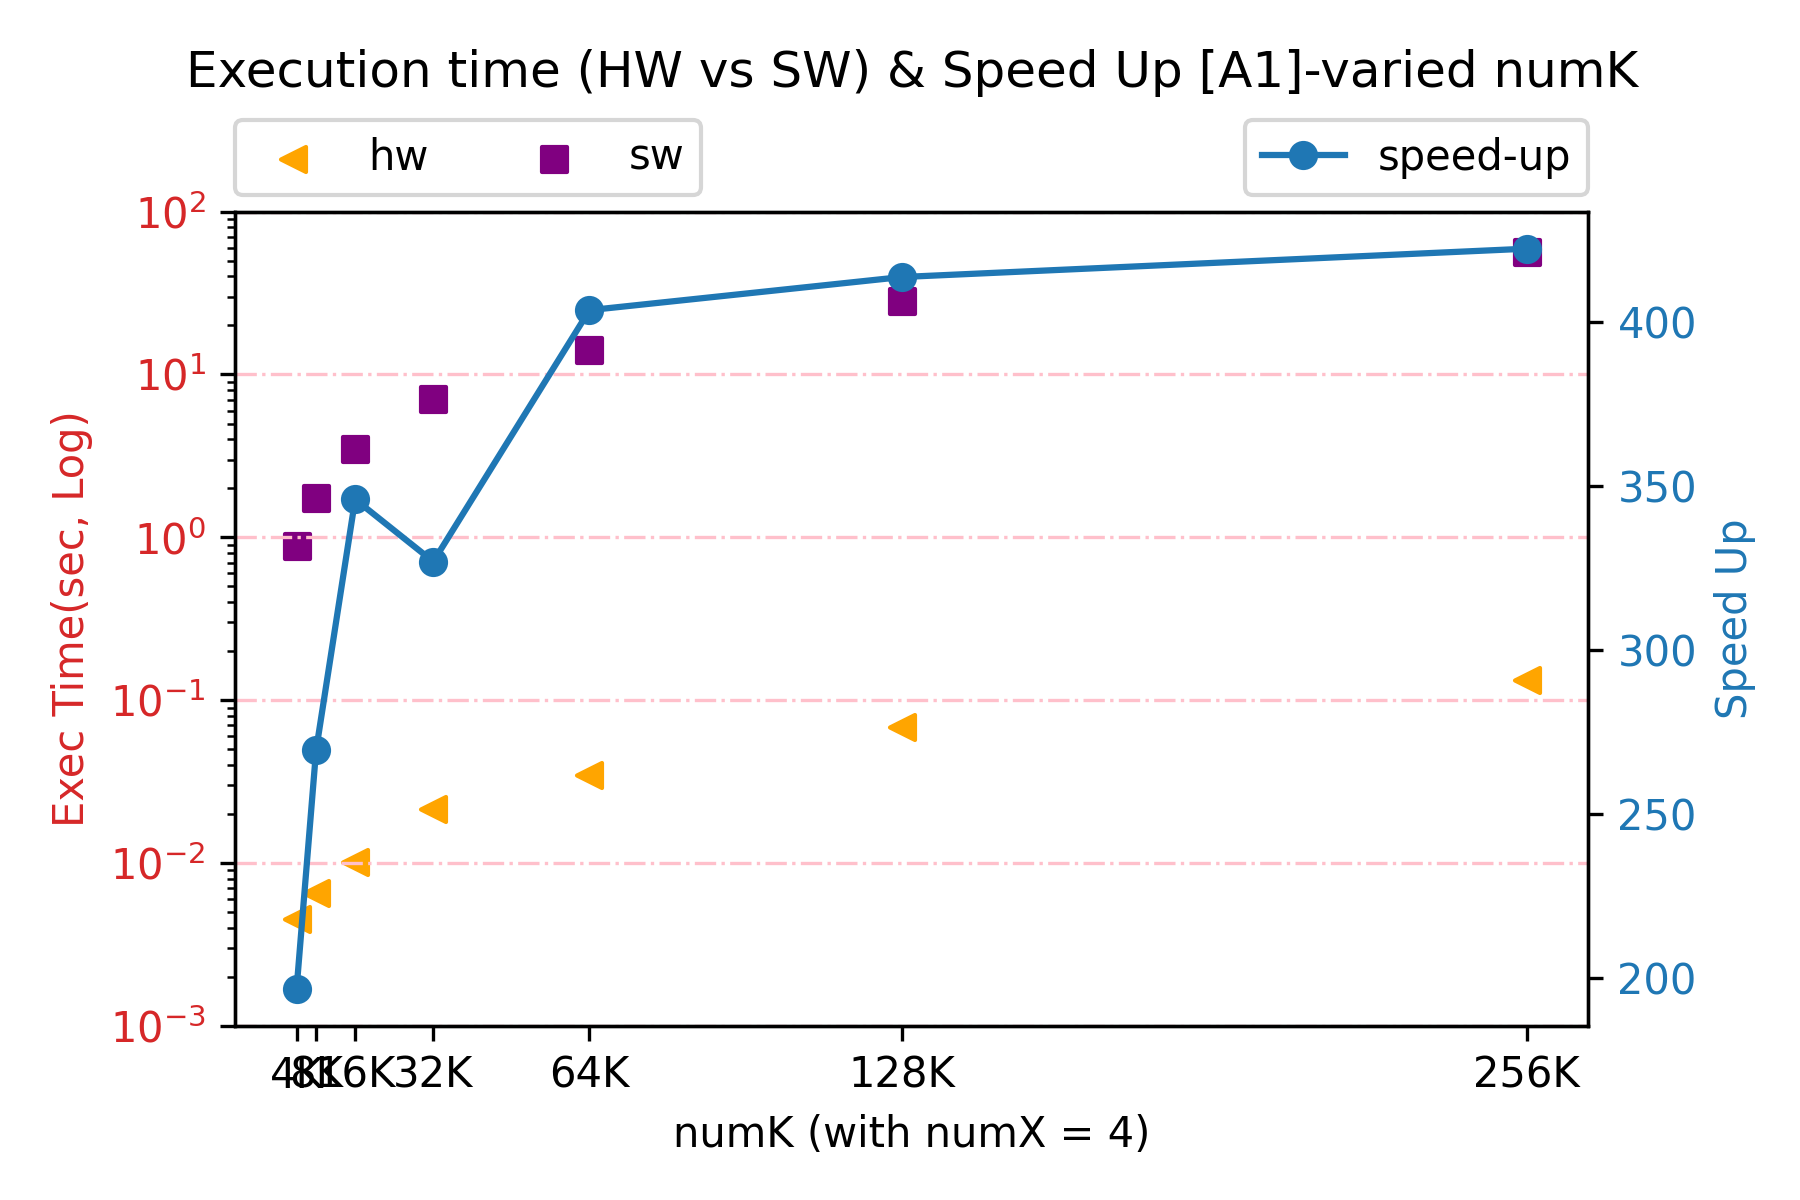
\includegraphics[width=\columnwidth]{figures/a1-vary-k.png}
    \caption{Latency with varying numK (numX=4)}
    \label{fig-a1-k}
\end{figure}
